%  We first introduce the concept of pushout from category theory in \hyperref[preliminaries:pushout]{Section~\ref*{preliminaries:pushout}}. 
%   Next, we discuss the double-pushout (DPO) rewriting in \hyperref[preliminaries:grs]{Section~\ref*{preliminaries:grs}}. 
%   Finally, we explore the concept of relative termination in \hyperref[preliminaries:relative_termination]{Section~\ref*{preliminaries:relative_termination}}. 
%   Additionally, we introduce the notion of a strongly monotonic measurable semiring in \hyperref[sec:strongly_monotonic_measurable_semiring]{Section~\ref*{sec:strongly_monotonic_measurable_semiring}}. 
%   The type graph, which is presented in \hyperref[sec:weighted_type_graph]{Section~\ref*{sec:weighted_type_graph}}, is weighted over this semiring.
  
In this section, we recall definitions related to the double-pushout approach to graph rewriting and relative termination, and we introduce strongly monotonic measurable semirings. For further details, we refer the reader to~\cite{konig2018tutorial,ehrig1997algebraic,habel2001double} for the DPO graph rewriting,~\cite{pierce1991basic, barr1990category} for category theory concepts, and~\cite{geser1990relative} for relative termination.
 
\subsection{Pushout}
\label{preliminaries:pushout}
\todo{Over-formalisation}
\begin{definition}[\cite{barr1990category}]
    \label{def:graph:unlabeled}
    An \textbf{unlabeled graph} \( G \) consists of a collection of \textbf{nodes} (also called \textbf{objects}) and a collection of \textbf{edges}\trackedtext{, each} equipped with a \textbf{source} (or \textbf{domain}) node and a \textbf{target} (or \textbf{codomain}) node. 
    For an unlabeled graph \( G \), we denote by \( G_0 \) its collection of nodes, \( G_1 \) its collection of edges, \( \operatorname{dom}:G_1{\to}G_0 \) the domain function, and \( \operatorname{cod}:G_1{\to}G_0 \) the codomain function. An unlabeled graph is \textbf{finite} if \( G_0 \) and \( G_1 \) are both finite sets.
    We write \( a: s \to t \) to indicate that \( a \) is a directed edge from \( s \) to \( t \).
\end{definition}   
\begin{definition}[Category~\cite{pierce1991basic, barr1990category}]
    \label{def:cat}
    A \textbf{category} is an unlabeled graph \( C \) together with a total function \( u : C_0 \mathop{\to} C_1 \) and a partial function \( \star: C_1 \mathop{\times} C_1 \mathop{\to} C_1 \) such that 
        (i) for all edges \( f:X \mathop{\to} Y \) and \( g:Y \mathop{\to} Z \), the edge \( f \mathop{\star} g :X \mathop{\to} Z \) is defined; 
        (ii) for every node \( X \), \( u(X) \) is an edge from \( X \) to \( X \);
        (iii) for every \( f:X \mathop{\to} Y \), we have \(u(X) \mathop{\star} f \mathop{=} f \mathop{=} f \mathop{\star} u(Y)\);
        (iv) for all edges \( f \), \( g \) and \(h\), we have \( (f \mathop{\star} g) \mathop{\star} h \mathop{=} f \mathop{\star} (g \mathop{\star} h) \) whenever either side is defined.
    Edges are called \textbf{morphisms}. The function $\star$ is called \textbf{composition}. For all \( X \mathop{\in} C_0 \), the edge \( u(X) \) is denoted \( \operatorname{id}_X \) and is called the \textbf{identity} of the object \( X \).
    % \( C \) is called the \textbf{underlying graph} of the category \( \mathcal{C} \).
\end{definition} 
\begin{notation}
    The composition of morphisms \( f : X \to Y \) and \( g : Y \to Z \) is written in diagrammatic order as \( f \star g \), rather than in functional order \( g \circ f \). 
    % The advantage is that, when reading from left to right, the morphisms appear in the same order as in the corresponding diagram, making the notation more intuitive for visual reasoning.
\end{notation}  
\begin{definition}[Monomorphism \cite{pierce1991basic,barr1990category}]
    \label{def:cat:homo}
    A morphism \( f : X \to Y \) is \textbf{monic} (or a \textbf{monomorphism}) if for all morphisms \( g \) and \( h \), if \( g \star f = h \star f \), then \( g = h \). A monomorphism is denoted by \( f : X \rightarrowtail Y \).
\end{definition} 

\begin{definition}[Span \cite{lowe2010graph}]
    A pair \( (\alpha : A \mathop{\to} B,~\beta : A \mathop{\to} C) \) of morphisms with a common domain is called a \textbf{span}, denoted by \( B \overset{\alpha}{\leftarrow} A \overset{\beta}{\rightarrow} C \).
\end{definition}

\begin{definition}[Cospan]
    An ordered pair \( (\beta' : B \to D,~\alpha' : C \to D) \) of morphisms with a common codomain is called a \textbf{cospan}, denoted by \( B \overset{\beta'}{\rightarrow} D \overset{\alpha'}{\leftarrow} C \). 
\end{definition} 


\begin{definition}[Diagram~\cite{barr1990category}]
    \label{def:cat:diagram}
    Let \( G \) be an unlabeled graph. A \textbf{diagram} (in \( \mathcal{C} \) of shape \( G \)) is a homomorphism of unlabeled graphs \( h : G \to C \) where \( C \) is the underlying unlabeled graph of the category \( \mathcal{C} \). A diagram is \textbf{commutative} if, for all nodes \( u \), \( v \), and any two paths from \( u \) to \( v \) in the unlabeled graph \( G \):

    \begin{center}
    \resizebox{12cm}{!}{
        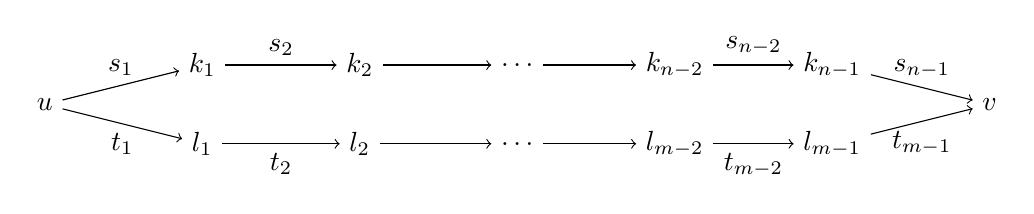
\begin{tikzpicture}
        \node (u) at (0,0) {\( u \)};
        \node (k1) at (2,0.5) {\( k_1 \)};
        \node (k2) at (4,0.5) {\( k_2 \)};
        \node (ketc) at (6,0.5) {\( \dots \)};
        \node (knm2) at (8,0.5) {\( k_{n-2} \)};
        \node (knm1) at (10,0.5) {\( k_{n-1} \)};
        \node (v) at (12,0) {\( v \)};
        \node (l1) at (2,-0.5) {\( l_1 \)};
        \node (l2) at (4,-0.5) {\( l_2 \)};
        \node (letc) at (6,-0.5) {\( \dots \)};
        \node (lnm2) at (8,-0.5) {\( l_{m-2} \)};
        \node (lnm1) at (10,-0.5) {\( l_{m-1} \)};
        \draw[->] (u) -- (k1) node [midway,above] {\( s_1 \)};
        \draw[->] (k1) -- (k2) node [midway,above] {\( s_2 \)};
        \draw[->] (k2) -- (ketc);
        \draw[->] (ketc) -- (knm2); 
        \draw[->] (knm2) -- (knm1) node[midway,above] {\( s_{n-2} \)}; 
        \draw[->] (knm1) -- (v) node[midway,above] {\( s_{n-1} \)}; 
        \draw[->] (u) -- (l1) node[midway,below] {\( t_1 \)};
        \draw[->] (l1) -- (l2) node[midway,below] {\( t_2 \)};
        \draw[->] (l2) -- (letc);
        \draw[->] (letc) -- (lnm2); 
        \draw[->] (lnm2) -- (lnm1) node[midway,below] {\( t_{m-2} \)}; 
        \draw[->] (lnm1) -- (v) node[midway,below] {\( t_{m-1} \)}; 
        \end{tikzpicture}
    }
    \end{center}
    \noindent
    the equality \( h(s_1) \star h(s_2) \star \dots  \star h(s_{n-1}) = h(t_1) \star h(t_2) \star \dots  \star h(t_{m-1}) \) holds.
\end{definition}

\begin{definition}[Pushout \cite{barr1990category}]
    \label{def:cat:po}
    \ \newline
\noindent
\begin{minipage}{0.7\textwidth}  
    A \textbf{pushout} of a span \( B \overset{\alpha}{\leftarrow} A \overset{\beta}{\rightarrow} C \), as shown on the right, is defined as a cospan \( B \overset{\beta'}{\rightarrow} D \overset{\alpha'}{\leftarrow} C \) such that \( \alpha \mathop{\star} \beta' \mathop{=} \beta \mathop{\star} \alpha' \), and for every cospan \( B \overset{\gamma'}{\rightarrow} E \overset{\gamma}{\leftarrow} C \), if \( \alpha \mathop{\star} \gamma' \mathop{=} \beta \mathop{\star} \gamma \) holds, then there exists a unique morphism \(\delta : D \mathop{\to} E\) such that \( \gamma' \mathop{=} \beta' \mathop{\star} \delta \) and \( \gamma \mathop{=} \alpha' \mathop{\star} \delta \).
\end{minipage}
\hfill
\begin{minipage}{0.299\textwidth}
    \hfill
\resizebox{0.9\textwidth}{!}{
           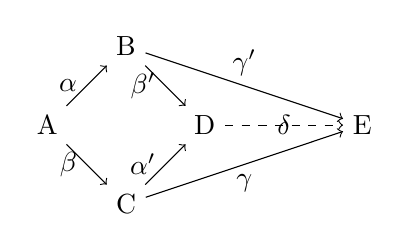
\begin{tikzpicture}
                \node (i) at (0,0) {A};
                \node (r) at (1,1) {B};
                \node (c) at (1,-1) {C};
                \node (h) at (2,0) {D};
                % \node () at (1,-1) {\( \Delta \)};
                \draw[->]  (i) -- (r) node [midway,left] {$ \alpha $};
                \draw[->] (c) -- (h) node [midway,left] {$ \alpha' $};
                \draw[->] (r) -- (h) node[midway, left] {$ \beta' $};
                \draw[->] (i) -- (c) node[midway, left] {$ \beta $};
                \node (d') at (4,0) {E};
                \draw[->] (c) -- (d') node [midway,below]{$ \gamma $};
                \draw[->] (r) -- (d') node [midway,above]{$ \gamma' $};
                \draw[->,dashed] (h) -- (d') node [midway]{$ \delta $};
            \end{tikzpicture}
}
\end{minipage}
The diagram involving \(\alpha\), \(\beta\), \(\alpha'\), and \(\beta'\) is referred to as the \textbf{pushout square}, \(D\) as the \textbf{pushout object}, and the existence of the unique morphism is known as the \textbf{universal mapping property of the pushout}.
\end{definition} 


\begin{notation}
    When the context makes it clear, a morphism \( h : A \mathop{\to} B \) will be denoted by \( h_{AB} \), and diagrams will be referred to by their nodes, as is standard in geometry. For example, the diagram involving the morphisms \( \alpha, \beta, \alpha', \beta' \) in Definition~\ref{def:cat:po} will be denoted by \( ACDB \) or \( ABDC \).
\end{notation}   

\subsection{DPO rewriting}
\label{preliminaries:grs}
\begin{definition}[Rewriting rule and match~\cite{corradini1997algebraic}]
  \label{def:grs:dpo_rule}
A \textbf{DPO rewriting rule} $\rho$ is a span \( L \overset{l}{\leftarrow} K \overset{r}{\rightarrow} R \), where \( K \) is the \textbf{interface}, \( L \) is the \textbf{left-hand-side graph}, denoted \( \operatorname{lhs}(\rho) \), and \( R \) is the \textbf{right-hand-side graph}, denoted \( \operatorname{rhs}(\rho) \). The rule is \textbf{monic} if $l$ and $r$ are both monic.
A match of the rule in an graph \( G \) is a morphism \( m: L \rightarrow G \).   
\end{definition}
   In this paper, we use examples from the category \textbf{Graph} of edge-labeled directed multigraphs (see~\cite{konig2018atutorial}) to illustrate the discussed concepts. 
\begin{example}
  \label{ex:grsaa}
  The injective DPO rule from \cite[Example 6]{bruggink2014termination} will be used to illustrate the concepts discussed throughout this paper.
  The rule can be visualized as follows:
  \begin{center} 
      \resizebox{0.7\textwidth}{!}{
      \begin{tikzpicture}
          \graphbox{$L$}{0mm}{0mm}{34mm}{15mm}{2mm}{-5mm}{
              \coordinate (o) at (0mm,-3mm); 
              \node[draw,circle] (l1) at ($(o)+(-10mm,0mm)$) {1};
              \node[draw,circle] (l2) at ($(l1)+(2,0)$) {2};
              \node[draw,circle] (l3) at ($(l1) + (1,0)$) {3};
              \draw[->] (l1) -- (l3) node[midway,above] {a};
              \draw[->] (l3) -- (l2) node[midway,above] {a};
          }     
          \graphbox{$K$}{40mm}{0mm}{24mm}{15mm}{2mm}{-5mm}{
              \coordinate (o) at (5mm,-3mm); 
              \node[draw,circle] (l1) at ($(o)+(-10mm,0mm)$) {1};
              \node[draw,circle] (l2) at ($(l1)+(1,0)$) {2};
              % \node[draw,circle] (l3) at ($(l1) + (1,0)$) {$\ $};
              % \draw[->] (l1) -- (l3) node[midway,above] {a};
              % \draw[->] (l3) -- (l2) node[midway,above] {a};
          }    
          \graphbox{$R$}{70mm}{0mm}{45mm}{15mm}{2mm}{-5mm}{
              \coordinate (o) at (-5mm,-3mm); 
              \node[draw,circle] (l1) at ($(o)+(-10mm,0mm)$) {1};
              \node[draw,circle] (l2) at ($(l1)+(3,0)$) {2};
              \node[draw,circle] (l3) at ($(l1) + (1,0)$) {4};
              \node[draw,circle] (l4) at ($(l1) + (2,0)$) {5};
              \draw[->] (l1) -- (l3) node[midway,above] {a};
              \draw[->] (l3) -- (l4) node[midway,above] {b};
              \draw[->] (l4) -- (l2) node[midway,above] {a};
          }    
          \node () at (37mm,-8mm) {$\overset{l}{\leftarrowtail}$};
          \node () at (67mm,-8mm) {$\overset{r}{\rightarrowtail}$};
          % \draw[>->] (51mm,2mm) -- (52mm,3mm);
      \end{tikzpicture}
      }
  \end{center}
\end{example}
\begin{definition}[DPO Rewriting step \cite{endrullis2024generalized_arxiv_v2}]
  \label{def:rewriting_step}
    \ \newline
    \noindent
    \begin{minipage}{0.72\textwidth}
      A DPO diagram $\delta$ is a diagram as shown on the right.
      This diagram $\delta$ is a witness for the \textbf{rewriting step} from \( G \) to \( H \) using the rule \( \rho \) and \textbf{match} \( m \), denoted \( G \Rightarrow_\rho^m H \) or \( G \Rightarrow_\rho^\delta H \). We denote $\operatorname{left}(\delta)$ and $\operatorname{right}(\delta)$ the pushout squares $KLGC$ and $KRHC$, respectively.
    \end{minipage}
    \hfill
    \begin{minipage}{0.28\textwidth}
          % \begin{center}
          \hfill
          \resizebox{0.85\textwidth}{!}{
          \begin{tikzpicture}
            % [node distance=11mm]
            \node (I) at (0,0) {$K$};
            \node (L) at (-2,0) {$L$};
            \node (R) at (2,0) {$R$};
            \node (G) at (-2,-2) {$G$};
            \node (C) at (0,-2) {$C$};
            \node (H) at (2,-2) {$H$};
            \draw [->] (I) to  node [midway,below] {$l$} (L);
            \draw [->] (I) to  node [midway,below] {$r$} (R);
            \draw [->] (L) to node [midway,right] {$m$} (G);
            \draw [->] (I) to node [midway,right] {$u$} (C);
            \draw [->] (R) to node [midway,left] {$m'$} (H);
            \draw [->] (C) to node [midway,above] {$l'$} (G);
            \draw [->] (C) to node [midway,above] {$r'$} (H);
            \node [at=($(I)!.5!(G)$)] {\normalfont PO};
            \node [at=($(I)!.5!(H)$)] {\normalfont PO};
          \end{tikzpicture}
        % \end{center}
        }
        \end{minipage}
  \end{definition}
\begin{example}
  \label{ex:rewriting_step_grs_aa}
  The DPO diagram below defines a rewriting step using the rule from Example~\ref{ex:grsaa}.
  \begin{center} 
      \resizebox{0.7\textwidth}{!}{
      \begin{tikzpicture}
          \graphbox{\( L \)}{0mm}{-3mm}{34mm}{12mm}{2mm}{2mm}{
              \coordinate (o) at (0mm,-8mm); 
              \node[draw,circle] (l1) at ($(o)+(-10mm,0mm)$) {1};
              \node[draw,circle] (l2) at ($(l1)+(2,0)$) {2};
              \node[draw,circle] (l3) at ($(l1) + (1,0)$) {3};
              \draw[] (l1) -- (l3) node[midway,above] {$a$};
              \draw[] (l3) -- (l2) node[midway,above] {$a$};
          } 
          \graphbox{\( K \)}{40mm}{-3mm}{34mm}{12mm}{2mm}{2mm}{
              \coordinate (o) at (0mm,-8mm); 
              \node[draw,circle] (l1) at ($(o)+(-10mm,0mm)$) {1};
              \node[draw,circle] (l2) at ($(l1)+(2,0)$) {2};
          }  
          \graphbox{\( R \)}{80mm}{-3mm}{45mm}{12mm}{2mm}{2mm}{
              \coordinate (o) at (-5mm,-8mm); 
              \node[draw,circle] (l1) at ($(o)+(-10mm,0mm)$) {1};
              \node[draw,circle] (l2) at ($(l1)+(3,0)$) {2};
              \node[draw,circle] (l3) at ($(l1) + (1,0)$) {4};
              \node[draw,circle] (l4) at ($(l1) + (2,0)$) {5};
              \draw[ ] (l1) -- (l3) node[midway,above] {$a$};
              \draw[ ] (l3) -- (l4) node[midway,above] {$b$};
              \draw[ ] (l4) -- (l2) node[midway,above] {$a$};
          }    
          \graphbox{\( G \)}{0mm}{-22mm}{34mm}{22mm}{2mm}{-3mm}{
              \coordinate (o) at (0mm,-3mm); 
              \node[draw,circle] (l1) at ($(o)+(-10mm,0mm)$) {1};
              \node[draw,circle] (l2) at ($(l1)+(2,0)$) {2};
              \node[draw,circle] (l3) at ($(l1) + (1,0)$) {3};
              \node[draw,circle] (l4) at ($(l2) + (0,-1)$) {6};
              \draw[] (l1) -- (l3) node[midway,above] {$a$};
              \draw[] (l3) -- (l2) node[midway,above] {$a$};
              \draw[ ] (l2) -- (l4) node[midway,right] {$a$};
              \node[draw,circle] (l6) at ($(l1) + (0,-1)$) {7};
              \draw[] (l1) -- (l6) node[midway,left] {$a$};
          }    
          \graphbox{\( C  \)}{40mm}{-22mm}{34mm}{22mm}{2mm}{-3mm}{
              \coordinate (o) at (0mm,-3mm); 
              \node[draw,circle] (l1) at ($(o)+(-10mm,0mm)$) {1};
              \node[draw,circle] (l2) at ($(l1)+(2,0)$) {2};
              \node[draw,circle] (l4) at ($(l2) + (0,-1)$) {6};
              \draw[ ] (l2) -- (l4) node[midway,right] {$a$};
              \node[ draw,circle] (l6) at ($(l1) + (0,-1)$) {7};
              \draw[ ] (l1) -- (l6) node[midway,left] {$a$};
          }    
          \graphbox{\( H \)}{80mm}{-22mm}{45mm}{22mm}{2mm}{-3mm}{
              \coordinate (o) at (-5mm,-3mm); 
              \node[draw,circle] (l1) at ($(o)+(-10mm,0mm)$) {1};
              \node[draw,circle] (l2) at ($(l1)+(3,0)$) {2};
              \node[draw,circle] (l3) at ($(l1) + (1,0)$) {4};
              \node[draw,circle] (l4) at ($(l1) + (2,0)$) {5};
              \node[ draw,circle] (l5) at ($(l2) + (0,-1)$) {6};
              \node[ draw,circle] (l6) at ($(l1) + (0,-1)$) {7};
              \draw[ ] (l1) -- (l6) node[midway,left] {$a$};
              \draw[] (l1) -- (l3) node[midway,above] {$a$};
              \draw[] (l3) -- (l4) node[midway,above] {$b$};
              \draw[ ] (l4) -- (l2) node[midway,above] {$a$};
              \draw[ ] (l2) -- (l5) node[midway,right] {$a$};
          }    
          \node () at (37mm,-8mm) {\( \leftarrowtail \)}; % K -> L
          \node () at (77mm,-8mm) {\( \rightarrowtail \)}; % K -> R
          \node () at (15mm,-18mm) {\( m\ \downarrowtail \)};
          \node () at (37mm,-33mm) {\( \leftarrowtail \)};
          \node () at (58mm,-18mm) {\( u\downarrowtail \)};
          \node () at (102mm,-18mm) {\( \downarrowtail \)};
          \node () at (77mm,-33mm) {\( \rightarrowtail \)}; % C -> H
      \end{tikzpicture}
      }
  \end{center}
\end{example}
DPO rewriting has several variants, depending on factors such as whether the matching morphism, the left-hand morphism, or the right-hand morphism is monic~\cite{habel2001double}, and whether the left pushout square is restricted~\cite{behr2021concurrency,behr2023fundamentals}. Since these restrictions can influence the termination properties of a DPO rewrite system,  we use the parametric definition presented in~\cite{EndrullisOverbeek2024Generalized} to encompass different DPO variants.
% \begin{definition}[DPO rewriting framework~\cite{endrullis2024generalized_arxiv_v2}]
%     A \emph{DPO rewriting framework} $\mathfrak{F}$ is a mapping of DPO rewriting rules to classes of DPO diagrams such that, for every DPO rule $\rho$, $\mathfrak{F}(\rho)$ is a class of DPO diagrams with top-span $\rho$.
    
%     The DPO rewriting relation $\mathop{\Rightarrow}_{\rho,\mathfrak{F}}$ induced by a DPO rewriting rule $\rho$ in $\mathfrak{F}$ is defined as follows: $G \mathop{\Rightarrow}_{\rho,\mathfrak{F}} H$ iff $G \mathop{\Rightarrow}_\rho^\delta H$ for some $\delta \mathop{\in} \mathfrak{F}(\rho)$. 
%     % for some $\delta \mathop{\in} \mathfrak{F}(\rho)$
%     The rewriting relation $\mathop{\Rightarrow}_{\mathcal{R},\mathfrak{F}}$ induced by a set $\mathcal{R}$ of DPO rewriting rules in $\mathfrak{F}$ is given by: $G \mathop{\Rightarrow}_{\mathcal{R},\mathfrak{F}} H$ iff $G \mathop{\Rightarrow}_{\rho,\mathfrak{F}} H$ for some $\rho \mathop{\in} \mathcal{R}$. When $\mathfrak{F}$ is clear from the context, we 
%     suppress $\mathfrak{F}$ and 
%     write $\mathop{\Rightarrow}_{\rho}$ and $\mathop{\Rightarrow}_{\mathcal{R}}$.
% \end{definition} 
\begin{definition}[Rewriting framework~\cite{endrullis2024generalized_arxiv_v2}]
    A \textbf{DPO rewriting framework} $\mathfrak{F}$ is a mapping of DPO rewriting rules to collections of DPO diagrams. Specifically, for every rule \( \rho \mathop{=} (L \overset{l}{\leftarrow} K \overset{r}{\rightarrow} R) \), the collection $\mathfrak{F}(\rho)$ consists of DPO diagrams of the form shown in Definition~\ref{def:rewriting_step}.

    The \textbf{DPO rewriting relation $\mathop{\Rightarrow}_{\rho,\mathfrak{F}}$ induced by a DPO rewriting rule $\rho$ in $\mathfrak{F}$} is defined as follows: $G \mathop{\Rightarrow}_{\rho,\mathfrak{F}} H$ iff $G \mathop{\Rightarrow}_\rho^\delta H$ for some $\delta \mathop{\in} \mathfrak{F}(\rho)$. 
    % for some $\delta \mathop{\in} \mathfrak{F}(\rho)$
     The \textbf{DPO rewriting relation $\mathop{\Rightarrow}_{\mathcal{R},\mathfrak{F}}$ induced by a set $\mathcal{R}$ of DPO rewriting rules in $\mathfrak{F}$} is given by: $G \mathop{\Rightarrow}_{\mathcal{R},\mathfrak{F}} H$ iff $G \mathop{\Rightarrow}_{\rho,\mathfrak{F}} H$ for some $\rho \mathop{\in} \mathcal{R}$. When $\mathfrak{F}$ is clear from the context, we 
    suppress $\mathfrak{F}$ and 
    write $\mathop{\Rightarrow}_{\rho}$ and $\mathop{\Rightarrow}_{\mathcal{R}}$.
  \end{definition}
\subsection{Relative termination}
  \label{preliminaries:relative_termination}
\begin{definition}[Rewriting sequence]
    Let \(\mathcal{R}\) be a set of rewriting rules. Let $\mathfrak{F}$ be a DPO rewriting framework.
    A \textbf{$(\mathcal{R},\mathfrak{F})$-rewriting sequence} is a finite sequence \(s_0,s_1,\hdots, s_m\) of objects such that \(s_n \mathop{\Rightarrow}_{\mathcal{R},\mathfrak{F}} s_{n+1}\) for each \( 0 \leq n \leq m-1\), or an infinite sequence \(s_0,s_1,\hdots\) of objects such that \(s_n \mathop{\Rightarrow}_{\mathcal{R},\mathfrak{F}} s_{n+1}\) for each \(n \mathop{\in} \mathbb{N}\).
    A $(\mathcal{R},\mathfrak{F})$-rewriting sequence from \( s_0 \) will be denoted as:
    \(
    s_0 \mathop{\Rightarrow}_{\mathcal{R},\mathfrak{F}} s_1 \mathop{\Rightarrow}_{\mathcal{R},\mathfrak{F}} s_2 \mathop{\Rightarrow}_{\mathcal{R},\mathfrak{F}} \cdots 
    \)
\end{definition}
\begin{definition}[Rewriting sequence]
    Let \(\mathcal{R}\) be a set of rewriting rules and let $\mathfrak{F}$ be a DPO rewriting framework.
    A \textbf{$(\mathcal{R},\mathfrak{F})$-rewriting sequence} is either a finite sequence \(s_0,s_1,\hdots, s_m\) of objects such that \(s_n \Rightarrow_{\mathcal{R},\mathfrak{F}} s_{n+1}\) for each \( 0 \leq n \leq m-1\), or an infinite sequence \(s_0,s_1,\hdots\) of objects such that \(s_n \Rightarrow_{\mathcal{R},\mathfrak{F}} s_{n+1}\) for each \(n \in \mathbb{N}\).
    A $(\mathcal{R},\mathfrak{F})$-rewriting sequence from \( s_0 \) will be denoted as:
    \(
    s_0 \Rightarrow_{\mathcal{R},\mathfrak{F}} s_1 \Rightarrow_{\mathcal{R},\mathfrak{F}} s_2 \Rightarrow_{\mathcal{R},\mathfrak{F}} \cdots 
    \)
\end{definition}

\begin{example}
    Consider the rewriting rules in~\autoref{fig:preliminaries:graph_transformation_rule_nonterminating}.
    \begin{figure}[hbtp]
        \centering
            \resizebox{0.85\textwidth}{!}{
                \begin{tikzpicture}[baseline=-3ex]
                    \graphbox{\( L \)}{0mm}{-3mm}{34mm}{15mm}{2mm}{2mm}{
                        \coordinate (o) at (0mm,-11mm); 
                        \node[draw,circle] (l1) at ($(o)+(-10mm,0mm)$) {1};
                        \node[draw,circle] (l2) at ($(l1)+(2,0)$) {2};
                        \node[draw,circle] (l3) at ($(l1) + (1,0)$) {3};
                        \draw[->] (l1) -- (l3) node[midway,above] {a};
                        \draw[->] (l3) -- (l2) node[midway,above] {b};
                    } 
            
                    \graphbox{\( K \)}{40mm}{-3mm}{34mm}{15mm}{2mm}{2mm}{
                        \coordinate (o) at (0mm,-11mm); 
                        \node[draw,circle] (l1) at ($(o)+(-10mm,0mm)$) {1};
                        \node[draw,circle] (l2) at ($(l1)+(2,0)$) {2};
                    }  
            
                    \graphbox{\( R \)}{80mm}{-3mm}{35mm}{15mm}{2mm}{2mm}{
                        \coordinate (o) at (-5mm,-11mm); 
                        \node[draw,circle] (l1) at ($(o)+(-10mm,0mm)$) {1};
                        % \node[draw,circle] (l2) at ($(l1)+(3,0)$) {2};
                        \node[draw,circle] (l3) at ($(l1) + (1,0)$) {4};
                        \node[draw,circle] (l4) at ($(l1) + (2,0)$) {2};
                        \draw[->] (l1) -- (l3) node[midway,above] {b};
                        \draw[->] (l3) -- (l4) node[midway,above] {a};
                        % \draw[->] (l4) -- (l2) node[midway,above] {a};
                    }    
                    \node () at (37mm,-10mm) {\( \leftarrowtail \)}; % K -> L
                    \node () at (77mm,-10mm) {\( \rightarrowtail \)}; % K -> R
                \end{tikzpicture}
                }
        \caption{}
        \label{fig:preliminaries:graph_transformation_rule_nonterminating}
    \end{figure} 
    A rewriting sequence using the rule with matches in red is shown in~\autoref{fig:preliminaries:sequence_of_transformation_infinite}.
       
        \begin{figure}[hbtp]
            \centering
          \resizebox{0.85\textwidth}{!}{
            \tikz
            [baseline=-0.5ex]
            { 
                \node (x) at (0,0) {$\bullet$};  
                \node (y) at (1,0) {$\bullet$};
                \node (z) at (0.5,0.86) {$\bullet$};
                \draw[->,red] (x) -- node[midway,below] {a} (y) ;
                \draw[->,red] (y) -- node[midway,right] {b} (z) ;
                \draw[->] (z) -- node[midway,left] {b} (x) ;
            } 
            $\Rightarrow$ 
            \tikz[baseline=-0.5ex]{ 
                \node (x) at (0,0) {$\bullet$};  
                \node (y) at (1,0) {$\bullet$};
                \node (z) at (0.5,0.86) {$\bullet$};
                \draw[->] (x) -- node[midway,below] {b} (y) ;
                \draw[->,red] (y) -- node[midway,right] {a} (z) ;
                \draw[->,red] (z) -- node[midway,left] {b} (x) ;
            }
            $\Rightarrow$ 
            \tikz[baseline=-0.5ex]{ 
                \node (x) at (0,0) {$\bullet$};  
                \node (y) at (1,0) {$\bullet$};
                \node (z) at (0.5,0.86) {$\bullet$};
                \draw[->,red] (x) -- node[midway,below] {b} (y) ;
                \draw[->] (y) -- node[midway,right] {b} (z) ;
                \draw[->,red] (z) -- node[midway,left] {a} (x) ;
            }
            $\Rightarrow$ 
            \tikz[baseline=-0.5ex]{ 
                \node (x) at (0,0) {$\bullet$};   
                \node (y) at (1,0) {$\bullet$};
                \node (z) at (0.5,0.86) {$\bullet$};
                \draw[->,red] (x) -- node[midway,below] {a} (y) ;
                \draw[->,red] (y) -- node[midway,right] {b} (z) ;
                \draw[->] (z) -- node[midway,left] {b} (x) ;
            }
          }
          \caption{}
          \label{fig:preliminaries:sequence_of_transformation_infinite}
        \end{figure}
\end{example}
We adapt the concept of relative termination~\cite{klop1987term,geser1990relative} to DPO rewriting.
\begin{definition}[Relative termination]
    \label{termination:def:relative_termination}
     Let $\mathcal{A}$ and $\mathcal{B}$ be sets of rewriting rules and let $\mathfrak{F}$ be a DPO rewriting framework. We say that $\Rightarrow_{\mathcal{A},\mathfrak{F}}$ is \textbf{terminating relative to} $\Rightarrow_{\mathcal{B}, \mathfrak{F}}$ if any infinite $(\mathcal{A} \cup \mathcal{B},\mathfrak{F})$-rewriting sequence has only a finite number of rewriting steps with rules in $\mathcal{A}$.
\end{definition}

\begin{example}
    Consider the rewriting system with two rules.
    
     
    \begin{figure}[hbtp]
     $\alpha$ = \resizebox{0.85\textwidth}{!}{ 
                \begin{tikzpicture}[baseline=-3ex]
                    \graphbox{\( L \)}{0mm}{-3mm}{34mm}{15mm}{2mm}{2mm}{
                        \coordinate (o) at (0mm,-11mm); 
                        \node[draw,circle] (l1) at ($(o)+(-10mm,0mm)$) {1};
                        \node[draw,circle] (l2) at ($(l1)+(2,0)$) {2};
                        % \node[draw,circle] (l3) at ($(l1) + (1,0)$) {3};
                        \draw[->] (l1) -- (l2) node[midway,above] {a};
                    } 
            
                    \graphbox{\( K \)}{40mm}{-3mm}{34mm}{15mm}{2mm}{2mm}{
                        \coordinate (o) at (0mm,-11mm); 
                        \node[draw,circle] (l1) at ($(o)+(-10mm,0mm)$) {1};
                        \node[draw,circle] (l2) at ($(l1)+(2,0)$) {2};
                    }  
            
                    \graphbox{\( R \)}{80mm}{-3mm}{35mm}{15mm}{2mm}{2mm}{
                        \coordinate (o) at (-5mm,-11mm); 
                        \node[draw,circle] (l1) at ($(o)+(-10mm,0mm)$) {1};
                        % \node[draw,circle] (l2) at ($(l1)+(3,0)$) {2};
                        % \node[draw,circle] (l3) at ($(l1) + (1,0)$) {4};
                        \node[draw,circle] (l4) at ($(l1) + (2,0)$) {2};
                        \draw[->] (l1) -- (l4) node[midway,above] {b};
                        % \draw[->] (l4) -- (l2) node[midway,above] {a};
                    }    
                    \node () at (37mm,-10mm) {\( \leftarrowtail \)}; % K -> L
                    \node () at (77mm,-10mm) {\( \rightarrowtail \)}; % K -> R
                \end{tikzpicture}
                }
 
     $\beta$ = \resizebox{0.85\textwidth}{!}{ 
                \begin{tikzpicture}[baseline=-3ex]
                    \graphbox{\( L \)}{0mm}{-3mm}{34mm}{15mm}{2mm}{2mm}{
                        \coordinate (o) at (0mm,-11mm); 
                        \node[draw,circle] (l1) at ($(o)+(-10mm,0mm)$) {1};
                        \node[draw,circle] (l2) at ($(l1)+(2,0)$) {2};
                        % \node[draw,circle] (l3) at ($(l1) + (1,0)$) {3};
                        \draw[->] (l1) -- (l2) node[midway,above] {a};
                    } 
            
                    \graphbox{\( K \)}{40mm}{-3mm}{34mm}{15mm}{2mm}{2mm}{
                        \coordinate (o) at (0mm,-11mm); 
                        \node[draw,circle] (l1) at ($(o)+(-10mm,0mm)$) {1};
                        \node[draw,circle] (l2) at ($(l1)+(2,0)$) {2};
                    }  
            
                    \graphbox{\( R \)}{80mm}{-3mm}{35mm}{15mm}{2mm}{2mm}{
                        \coordinate (o) at (-5mm,-11mm); 
                        \node[draw,circle] (l1) at ($(o)+(-10mm,0mm)$) {1};
                        % \node[draw,circle] (l2) at ($(l1)+(3,0)$) {2};
                        % \node[draw,circle] (l3) at ($(l1) + (1,0)$) {4};
                        \node[draw,circle] (l4) at ($(l1) + (2,0)$) {2};
                        \draw[->] (l1) -- (l4) node[midway,above] {a};
                        % \draw[->] (l4) -- (l2) node[midway,above] {a};
                    }    
                    \node () at (37mm,-10mm) {\( \leftarrowtail \)}; % K -> L
                    \node () at (77mm,-10mm) {\( \rightarrowtail \)}; % K -> R
                \end{tikzpicture}
                }
    \end{figure}
    The rewriting system is not terminating because of the rule $\beta$, but the rule $\alpha$ is terminating relative to $\beta$ because it can only be applied finitely many times in any rewriting sequence that uses $\alpha$ and $\beta$.
\end{example}
% The concept of relative termination generalizes the notion of uniform termination of DPO graph rewriting systems which is a fundamental property of algorithms because many other properties are based on it. Given a set of rules, the uniform termination means that any rewriting sequence using these rules has a finite length. Uniform termination is undecidable in general~\cite{plump1998terminationundecidable}. It is a fundamental property of rewriting systems because it is a prerequisite for reasoning about the correctness of algorithms based on these systems.
% For example, there is no point to talk about the correctness of the result of an algorithm if the algorithm does not terminate. In the context of graph rewriting, termination means that any graph can not be transformed indefinitely by applying rewriting rules. Plump has shown that termination of DPO graph rewriting systems is undecidable in general~\cite{plump1998terminationundecidable}.

 
\subsection{Strongly monotonic measurable semiring}
\label{sec:strongly_monotonic_measurable_semiring}
A commutative semiring is an algebraic structure (see~\cite{bruggink2015proving}\cite{endrullis2024generalized_arxiv_v2}). In this work, we adapt the concept of an ordered semiring from~\cite{endrullis2024generalized_arxiv_v2}. 
The key difference is that the semiring is required to be equipped with a homomorphism to the extended real numbers instead of being well-founded.
Throughout the remainder of this article, $<$ and $\leq$ denote the canonical irreflexive and reflexive orders on the set of extended real numbers $\overline{\mathbb{R}} = \mathbb{R} \cup \{-\infty, +\infty\}$.
\begin{definition}[Strongly monotonic measurable semiring]
    \label{def:real_strongly_monotonic_semiring}
    A \textbf{strongly monotonic measurable semiring} $(S, \oplus, \odot, 0, 1, \prec, \mu)$ consists of
    \begin{itemize} 
        \item A commutative semiring $(S, \oplus, \odot, 0, 1)$,
        \item A non-empty irreflexive order $\prec$ on $S$,
        \item A homomorphism $\mu : (S, \prec) \to ( \overline{\mathbb{R}}, < )$,
    \end{itemize}
    such that $0 \neq 1$ and for all $x,y,z,w \in S$, for all $\delta \in \mathbb{R}_{\geq 0}$, we have
        \begin{align*}
            1 \preceq x \land 1 \preceq y 
            &\Rightarrow
            1 \preceq x \oplus y
            &\tag{S0} \label{ax:s0} 
            \\ 
            x \preceq x' \land y \preceq y' 
            &\Rightarrow
            x \oplus y \preceq x' \oplus y'
            &\tag{S1} \label{ax:s1} 
            \\   
            % x < y  
            % &\Rightarrow
            % x \oplus z \leq y \oplus z 
            % \tag{S1} \label{eq:ordered_semiring_plus_monotonic} 
            % \\ w
            x \prec x' \land y \prec y'  
            &\Rightarrow
            x \oplus y \prec x' \oplus y'
            &\tag{S2} \label{ax:s2} 
            \\
            \delta + \mu(x) < \mu(y) \land \delta + \mu(z) < \mu(w)
            &\Rightarrow
            \delta + \mu(x \oplus z) < \mu(y \oplus w)
            &\tag{S3} \label{ax:s2'}
            \\
            x \preceq x'
            &\Rightarrow 
            x \odot y \preceq x' \odot y 
            &\tag{S4} \label{ax:s3} 
            \\
            x \prec x' \land y \neq 0 
            &\Rightarrow
            x \odot y \prec x' \odot y
            &\tag{S5} \label{ax:s4}
            \\ 
            \delta + \mu(x) < \mu(y) \land 1 \preceq z \neq 0
            &\Rightarrow
            \delta + \mu(x \odot z) < \mu(y \odot z)
            &\tag{S6} \label{ax:s4'}
            \\
            \delta+ \mu(x) < \mu(x') \land y \neq 0
            &\Rightarrow
            \mu(x \odot y) < \mu(x' \odot y)
            &\tag{S7} \label{ax:s4''}
        %    \\
            % \\
            % 1 \leq z \neq 0 \land X < Y  
            % &\Rightarrow
            % \exists \mu(x * z) < \mu( y * z)
            % \tag{S101} \label{eq:strongly_ordered_measurable_semiring_lt_preserved_neq0_geq1}  
        %      \\     
        %     a + X < Y \land z \neq 0 
        %    &\Rightarrow
        %    \exists b> 0. b + \mu(x* z) < \mu(y * z) 
        %    \tag{S3} \label{eq:ordered_semiring_times_stable_under_mesure} 
        \end{align*}
        where $\preceq$ denotes the reflexive closure of $\prec$. The semiring is a \textbf{strictly monotonic measurable semiring} if it additionally satisfies 
    \begin{flalign*}
        \hspace{4.5cm} x \prec x' 
        &\Rightarrow
        x \oplus y \prec x' \oplus y 
        &\tag{S8} \label{ax:s5} 
        \\
        \delta + \mu(x) < \mu(x')
        &\Rightarrow
        \delta + \mu(x \oplus y) < \mu(x' \oplus y)
        &\tag{S9} \label{ax:s5'}
    \end{flalign*}
\end{definition} 
\begin{example} 
    % The real tropical semiring $\mathfrak{T}' = (\mathbb{R} \cup \{+\infty\}, \min,+,+\infty, 0_\mathbb{R},<,\operatorname{id}_{\mathbb{R} \cup \{+\infty\}})$ has domain $\mathbb{R} \cup \{+\infty\}$, the binary function symbol $\oplus$ interpreted by $\min$ and the binary function symbol $\odot$ interpreted by $+$, the constant symbols $0_s$ and $1_s$ interpreted by $+\infty$ and $0_\mathbb{R}$, respectively, the binary relation symbol $\prec$ interpreted by the canonical order $<$ on $\mathbb{R} \cup \{+\infty\}$, and the unary function symbol $\mu$ interpreted by the identity function on $\mathbb{R} \cup \{+\infty\}$. The real tropical semiring is a strongly monotonic measurable semiring. It is not strictly monotonic measurable because $2 < 3$ but $2 \oplus 2 = \min(2,2) = 2 \not < 2 = \min(3,2) = 3 \oplus 2$.

     The real tropical semiring $\mathfrak{T}' = (\mathbb{R} \cup \{+\infty\}, \min,+_\mathbb{R},+\infty, 0_\mathbb{R},<_\mathbb{R},\operatorname{id}_{\mathbb{R} \cup \{+\infty\}})$ is an instance of the strongly monotonic measurable semiring where
     \begin{flalign*}
         S & \mapsto \mathbb{R} \cup \{+\infty\}
         \\
         \oplus & \mapsto \min
         \\
         \odot & \mapsto +_\mathbb{R}
         \\
         0_s & \mapsto +\infty
         \\
         1_s & \mapsto 0_\mathbb{R}
         \\
         \prec & \mapsto <_\mathbb{R}
         \\
         \mu & \mapsto \operatorname{id}_{\mathbb{R} \cup \{+\infty\}}
     \end{flalign*}

    It is a strongly monotonic measurable semiring but not strictly monotonic measurable, because we have $2 <_\mathbb{R} 3$ but $2 \oplus 2 = \min(2,2) = 2 \not <_\mathbb{R} 2 = \min(3,2) = 3 \oplus 2$.
\end{example}
\begin{example}
    % The real arctic semiring $\mathfrak{A}' = (\mathbb{R} \cup \{-\infty\},\max,+,-\infty, 0_\mathbb{R},<,\operatorname{id}_{\mathbb{R} \cup \{-\infty\}})$ has domain $\mathbb{R} \cup \{-\infty\}$, the binary function symbol $\oplus$ interpreted by $\max$ and the binary function symbol $\odot$ interpreted by $+$, the constant symbols $0_s$ and $1_s$ interpreted by $-\infty$ and $0_\mathbb{R}$, respectively, the binary relation symbol $\prec$ interpreted by the canonical order $<$ on $\mathbb{R} \cup \{-\infty\}$, and the unary function symbol $\mu$ interpreted by the identity function on $\mathbb{R} \cup \{-\infty\}$. The real arctic semiring is a strongly monotonic measurable semiring. It is not strictly monotonic measurable because $2 < 3$ but $2 \oplus 3 = \max(2,3) = 3 \not < 3 = \max(3,3) = 3 \oplus 3$.
    The real arctic semiring $\mathfrak{A}' = (\mathbb{R} \cup \{-\infty\},\max,+_\mathbb{R},-\infty, 0_\mathbb{R},<_\mathbb{R},\operatorname{id}_{\mathbb{R} \cup \{-\infty\}})$ is an instance of the strongly monotonic measurable semiring where
    \begin{flalign*}
        S & \mapsto \mathbb{R} \cup \{-\infty\}
        \\
        \oplus & \mapsto \max
        \\
        \odot & \mapsto +_\mathbb{R}
        \\
        0_s & \mapsto -\infty
        \\
        1_s & \mapsto 0_\mathbb{R}
        \\
        \prec & \mapsto <_\mathbb{R}
        \\
        \mu & \mapsto \operatorname{id}_{\mathbb{R} \cup \{-\infty\}}
    \end{flalign*}
    It is a strongly monotonic measurable semiring but not strictly monotonic measurable, because $2 <_\mathbb{R} 3$ but $2 \oplus 3 = \max(2,3) = 3 \not <_\mathbb{R} 3 = \max(3,3) = 3 \oplus 3$.
%    The real arctic semiring: $\mathfrak{A}' = (\mathbb{R} \cup \{-\infty\},\max,+,-\infty, 0,<,\operatorname{id}_{\mathbb{R} \cup \{-\infty\}})$.
\end{example}
\begin{example}
    The real arithmetic semiring $\mathfrak{N}' = (\mathbb{R}^+,+_\mathbb{R},*_\mathbb{R},0_\mathbb{R},1_\mathbb{R},<,\operatorname{id}_{\mathbb{R}^+})$ is an instance of the strongly monotonic measurable semiring where
    \begin{flalign*}
        S & \mapsto \mathbb{R}^+
        \\
        \oplus & \mapsto +_\mathbb{R}
        \\
        \odot & \mapsto *_\mathbb{R}
        \\
        0_s & \mapsto 0_\mathbb{R}
        \\
        1_s & \mapsto 1_\mathbb{R}
        \\
        \prec & \mapsto <_\mathbb{R}
        \\
        \mu & \mapsto \operatorname{id}_{\mathbb{R}^+}
    \end{flalign*}
    It is a strictly monotonic measurable semiring. 
    % The real arithmetic semiring $\mathfrak{N}' = (\mathbb{R}^+,+,*,0_\mathbb{R},1_\mathbb{R},<,\operatorname{id}_{\mathbb{R}^+})$ has as domain the set $\mathbb{R}^+$ of positive real numbers, the binary function symbol $\oplus$ interpreted by $+$ and the binary function symbol $\odot$ interpreted by $*$, the constant symbols $0_s$ and $1_s$ interpreted by $0_\mathbb{R}$ and $1_\mathbb{R}$, respectively, the binary relation symbol $\prec$ interpreted by the canonical order $<$ on $\mathbb{R}^+$, and the unary function symbol $\mu$ interpreted by the identity function on $\mathbb{R}^+$. The real arithmetic semiring is a strictly monotonic measurable semiring. 
\end{example}
\begin{example} 
    \label{example:real_semirings}
    The natural tropical semiring $\mathfrak{T} = (\mathbb{N} \cup \{+\infty\},\min,+_{\mathbb{N}},+\infty, 0_\mathbb{N}, <_{\mathbb{N}} , \operatorname{id}_{\mathbb{N} \cup \{+\infty\}})$ is an instance of the strongly monotonic measurable semiring where
    \begin{flalign*}
        S & \mapsto \mathbb{N} \cup \{+\infty\}
        \\
        \oplus & \mapsto \min
        \\
        \odot & \mapsto +_\mathbb{N}
        \\
        0_s & \mapsto +\infty
        \\
        1_s & \mapsto 0_\mathbb{N}
        \\
        \prec & \mapsto <_\mathbb{N}
        \\
        \mu & \mapsto \operatorname{id}_{\mathbb{N} \cup \{+\infty\}}
    \end{flalign*}
    The natural arctic semiring $\mathfrak{A} = (\mathbb{N} \cup \{-\infty\},\max,+_{\mathbb{N}},-\infty, 0_\mathbb{N},<_{\mathbb{N}}, \operatorname{id}_{\mathbb{N} \cup \{-\infty\}})$ is an instance of the strongly monotonic measurable semiring where
    \begin{flalign*}
        S & \mapsto \mathbb{N} \cup \{-\infty\}
        \\
        \oplus & \mapsto \max
        \\
        \odot & \mapsto +_\mathbb{N}
        \\
        0_s & \mapsto -\infty
        \\
        1_s & \mapsto 0_\mathbb{N}
        \\
        \prec & \mapsto <_\mathbb{N}
        \\
        \mu & \mapsto \operatorname{id}_{\mathbb{N} \cup \{-\infty\}}
    \end{flalign*}  
    The natural arithmetic semiring $\mathfrak{N} = (\mathbb{N},+_\mathbb{N},*,0_\mathbb{N},1_\mathbb{N},<_\mathbb{N},\operatorname{id}_\mathbb{N})$ is an instance of the strictly monotonic measurable semiring where
    \begin{flalign*}
        S & \mapsto \mathbb{N}
        \\
        \oplus & \mapsto +_\mathbb{N}
        \\
        \odot & \mapsto *_\mathbb{N}
        \\
        0_s & \mapsto 0_\mathbb{N}
        \\
        1_s & \mapsto 1_\mathbb{N}
        \\
        \prec & \mapsto <_\mathbb{N}
        \\
        \mu & \mapsto \operatorname{id}_\mathbb{N}
    \end{flalign*}
\end{example}

% \begin{notation} 
%     \label{def:bigodot}
% Let $(S, \oplus, \odot, 0_s, 1_s)$ be a semiring. We extend naturally the binary operations $\oplus$ and $\odot$ to finite sets $E \subseteq S$ by letting
%     \begin{itemize}
%         \item $\bigodot \emptyset \overset{\operatorname{def}}{=} 1_s$ and $\bigodot \left( E \cup \{x\} \right) \overset{\operatorname{def}}{=} \left( \bigodot E \right) \odot x$;
%         \item $\bigoplus \emptyset \overset{\operatorname{def}}{=} 0_s$ and $\bigoplus \left( E \cup \{x\} \right) \overset{\operatorname{def}}{=} \left( \bigoplus E \right) \oplus x$.
%     \end{itemize}
% %  \begin{flalign*}
% %     \bigodot \emptyset &\overset{\operatorname{def}}{=} 1_s
% % \\
% %     \bigodot \left( E \cup \{x\} \right) &\overset{\operatorname{def}}{=} \left( \bigodot E \right) \odot x
% %     \\
% %     \bigoplus \emptyset &\overset{\operatorname{def}}{=} 0_s
% %     \\
% %         \bigoplus \left( E \cup \{x\} \right) &\overset{\operatorname{def}}{=} \left( \bigoplus E \right) \oplus x
% % \end{flalign*}
% \end{notation}

% \textcolor{blue}{\begin{remark}
%     \label{remark:diff_measurable_semiring}
% A strongly monotonic measurable semiring differs from a well-founded strongly monotonic semiring in~\cite{endrullis2024generalized} in four ways:
% \begin{enumerate}[label=(\arabic*),noitemsep]
%     \item Replacing well-foundedness with the homomorphism~$\mu$ and introducing Axioms \eqref{ax:s2'}, \eqref{ax:s4'}, and \eqref{ax:s4''}. This modification enables the use of non-well-founded semirings (e.g., as in~\autoref{example:real_semirings}).
%     % \item Removing the condition $1_S \preceq y$ from the original Axioms~(S3) and~(S4)\todo{This is not helpful}, resulting in our Axioms~(S4) and~(S5). This relaxation allows inclusion of elements smaller than $1_S$, as motivated in~\autoref{remark:greater_than_1}.
%     \item Adding Axiom~\eqref{ax:s0}. This technical adjustment ensures that if every $\mathcal{T}$-valued element of a type graph (see~\autoref{def:weighted_type_graph}) has a weight greater than $1_S$, then all objects subject to rewriting inherit this property.
%     \item Defining $\preceq$ as the reflexive closure of $\prec$ to simplify the theory. This is motivated by the fact that concrete semirings proposed in prior work and our paper satisfy this property.
% \end{enumerate} 
% \end{remark}}